La radiación ionizante es una herramienta moderna fundamental en el tratamiento de varias patologías. Su uso en medicina data desde la década de 1890, época en la que Roentgen reportó el descubrimiento de los rayos X y su capacidad de generar una imagen de los tejidos humanos internos de una forma efectiva, pero insegura por el desconocimiento parcial de los fenómenos involucrados. Gracias al desarrollo de la física detrás de estos fenómenos radiativos y al estudio de sus efectos sobre tejidos biológicos, se han logrado refinar estas herramientas para aplicaciones más sofisticadas como la radioterapia.\\

La eficiencia de estas herramientas en el tratamiento de enfermedades puede verse opacada por los grandes riesgos que se presentan cuando esta radiación no se aplica de manera segura. Por lo tanto, se hace necesario garantizar la seguridad en el uso de estos procedimientos, para lo cual es imprescindible la comprensión de los fenómenos físicos involucrados. Con este entendimiento es posible establecer protocolos de entrega de radiación y verificación de la misma que aseguren la máxima protección para todos los seres vivos que interactúan con ella. A continuación se expondrá un resumen de la teoría involucrada en estos procesos, así como algunos de los métodos que se usan en la actualidad para los propósitos antes mencionados.  \\

La radiación ionizante se refiere a aquellos haces de partículas con la capacidad de excitar o ionizar los átomos de la materia con la que interactúa. Para lograr este efecto se requieren energías de por lo menos 25 eV, que es la energía promedio con la cual están ligados al átomo los electrones en la capa de valencia. Por lo tanto, para que cierto haz de radiación electromagnética sea ionizante, este debe tener una longitud de onda no mayor a 320 nm, aproximadamente. \\

Los principales tipos de radiaciones ionizantes son los \textit{rayos} X, \textit{rayos }$\gamma$, haces de electrones libres, haces de neutrones y haces de partículas pesadas. Estos se pueden caracterizar por el tipo de partículas que son las portadoras de la energía y tienen propiedades particulares en cuanto a su poder de penetración.\\

Los rayos X y rayos $\gamma$ son radiación cuya energía es transportada por fotones. Los rayos X son radiación electromagnética emitida por partículas cargadas en transiciones atómicas, en cuyo caso se denominan rayos X característicos, o en procesos de Bremsstrahlung, en donde una partícula cargada es desacelerada por un campo columbiano de otra partícula cargada. Por lo general tienen energías de entre  0.1 KeV hasta varios MeV dependiendo del proceso de generación. Los rayos $\gamma$ son radiación electromagnética producida por núcleos atómicos en un proceso de decaimiento radiactivo o procesos de aniquilación materia anti-materia, su magnitud de energía generalmente está en el rango de MeV.\\

En los tipos restantes de radiación ionizante, la energía es transportada por partículas con masa. En el caso de electrones, estos pueden ser producidos en un proceso nuclear, en cuyo caso se denominan rayos $\beta$ o en colisiones de partículas cargadas, en cuyo caso de denominan rayos $\delta$. Este tipo de haces pueden ser generados en aceleradores lineales(\textit{linacs}) para múltiples propósitos. Los haces de partículas pesadas son por lo general obtenidos en procesos de aceleración en campos columbianos o como decaimiento radiactivo, en tal caso la energía es transportada por núcleos atómicos pesados, como las partículas $\alpha$. Finalmente, los haces de neutrones son haces en los que la energía es transportada por estas partículas sin carga emitidas en procesos nucleares. \\

Todos estos tipos de radiación interactúan con la materia, sin embargo, lo hacen de diferentes maneras. Se dice que un haz de radiación es directamente ionizante si la energía que se imprime a la materia se transmite directamente mediante interacciones columbianas en la trayectoria de la partícula, como en el caso de los haces de partículas cargadas. Por otro lado, se dice que un haz de radiación es indirectamente ionizante si la energía se transmite a las partículas cargadas del medio mediante otro tipo de procesos que serán discutidos posteriormente, como es el caso de los rayos X y rayos $\gamma$, que transmiten su energía mediante tres procesos principales, el efecto fotoeléctrico, el efecto compton y la producción de pares.\\

\section{Aceleradores lineales y radioterapia}
Existen múltiples usos para la radiación ionizante anteriormente caracterizada, entre ellos muchas aplicaciones médicas de diversa índole. A continuación se presenta un resumen de la producción y caracterización de radiación ionizante en aceleradores lineales y su uso en radioterapia. 
\subsection{Linac}
Existen diversos tipos de aceleradores creados para investigación en física nuclear y de altas energías, la mayoría de los cuales ha encontrado algún uso en aplicaciones médicas. Sin duda el tipo de acelerador más usado en esta área es el acelerador lineal(linac), en donde a través de campos eléctricos se aceleran partículas cargadas en movimiento rectilíneo. \\

Existen múltiples tecnologías que usan este tipo de dispositivos, como aquellas usadas en imágenes diagnosticas mediante rayos X, cristalografía o espectroscopia. Pero de entre ellas, la que más destaca y en donde se concentran los mayores esfuerzos de investigación en física médica es la aplicación de radiación ionizante producida en linacs con propósitos de radioterapia. \\

A diferencia de los aceleradores lineales usados en investigación de altas energías, los aceleradores que se usan para el tratamiento de cáncer son compactos y están diseñados para emitir un haz de radiación desde varias direcciones que llegan a un paciente, a quien se quiere irradiar con dosis concentrada en masas anormales, conservando la mayor cantidad de tejido sano posible.\\

Los aceleradores lineales convencionales usados en radioterapia aceleran electrones a energías entre 4 y 25 MeV, teniendo la opción de generar rayos X con estos electrones acelerados en este mismo intervalo de energía. Para lograr esta producción de radiación ionizante se tienen varias etapas en la máquina que se describen a continuación. En la figura \ref{fig:acelerador} se presenta un esquema de las múltiples secciones físicas en donde se desarrollan estas etapas.\\
\begin{figure}[H]
	\centering
	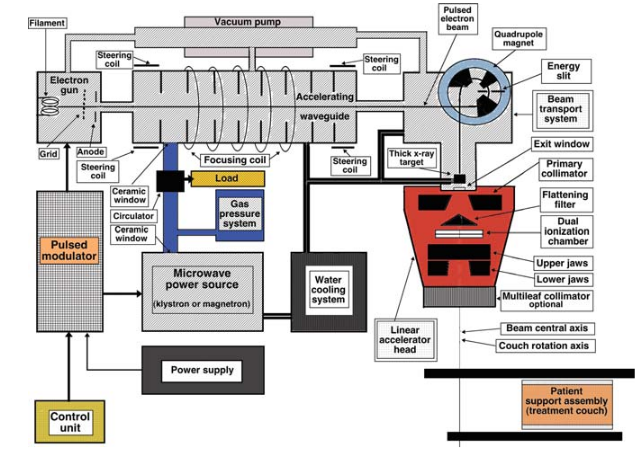
\includegraphics[width=0.9\linewidth]{images/linalc.png}
	\caption{Acelerador lineal típico usado en radioterapia \cite{podgorsak}}
	\label{fig:acelerador}
\end{figure}

\textbf{Etapa de producción de electrones}\\
La primera etapa en la generación del haz de electrones es su producción. El proceso de obtener electrones libres lo realiza 

\textbf{Etapa de generación de microondas}\\

\textbf{Etapa de aceleración en guía de onda}\\

\textbf{Etapa de direccionamiento de haz}\\

\textbf{Etapa de producción de rayos X}\\

\textbf{Etapa de colimación y filtrado}\\

\textbf{Mecanismos de soporte al funcionamiento}\\

\subsection{Procedimientos en radioterapia}

       


\section{Interacción radiación y partículas cargadas con materia}
\subsection{Interacción de fotones con materia}
Ahora, una vez determinadas las unidades con las que se medirá la radiación absorbida, es necesario establecer los mecanismos mediante los cuales esta interactúa con la materia y deposita energía en ella. Por lo tanto, a continuación se expondrán los procesos en los cuales los fotones depositan energía en los átomos y se presentará una manera de cuantificar este proceso numéricamente.  \\

Una partícula de un haz de radiación sin carga tiene alta probabilidad de pasar por una lámina delgada de algún material sin perder energía, mientras que un haz de partículas cargadas probablemente pierda parte o la totalidad de su energía. Ambos procesos hacen parte importante del proceso de transmisión de energía a la materia por parte de un haz de radiación. En esta sección estudiaremos los procesos mediante los cuales los fotones depositan energía.\\

\noindent
\textbf{Atenuación exponencial}\\


Consideremos un haz mono-energético de partículas sin carga que incide perpendicularmente en la superficie de un material de espesor $L$. Si inicialmente existen $N_0$ partículas en el haz, después de atravesar el material alguna proporción de estos habrá sido absorbida en alguna de las diversas interacciones que pueden ocurrir con las partículas cargadas en el medio. En una primera aproximación, consideramos el caso ideal en que ninguna radiación secundaria es producida, es decir, las partículas del haz o bien son absorbidas completamente, o bien pasan a través sin perder nada de su energía.\\

Para dar cuenta de este efecto de absorción general mediante diferentes mecanismos, se propone el modelo de atenuación exponencial, en el que se modela el cambio en el numero de partículas en el haz $dN$ mediante la relación
\begin{equation}
	dN=-\mu N dl,
\end{equation}  
donde $\mu$ es denominado el \textit{coeficiente de atenuación lineal} y está asociado a la probabilidad de que una partícula del haz sea absorbida en su trayecto por una distancia $dl$. Además, si esta cantidad se divide por la densidad $\rho$ del medio de atenuación, se obtiene el coeficiente másico de atenuación $\mu/\rho$.\\

Integrando esta relación entre $0$ y el espesor $L$ del material, obtenemos la relación
\begin{equation}
	N=N_0 e^{-\mu L},
\end{equation}
que es denominada la ley de atenuación exponencial, que da cuenta del número de partículas que no fueron absorbidas por el medio en su recorrido por el material de espesor $L$.\\

Para determinar este coeficiente asociado a la probabilidad de absorción, es necesario estudiar los mecanismos principales en los que se transfiere o deposita energía de un haz de partículas sin carga. En el contexto de radioterapia, existen tres principales mecanismos de transmisión de energía  de fotones a partículas con masa. A continuación se relacionan estos y una descripción de cómo modifican este coeficiente de atenuación.\\

\noindent
\textbf{Dispersión elástica e ineslástica}\\

Los procesos de dispersión se dan cuando un fotón incidente con cierta energía interactúa directamente con el átomo y no es absorbido por este. Existen dos tipos de dispersión, la primera es la dispersión elástica o de Rayleigh, en la cual el fotón es dispersado elásticamente, es decir, con un traspaso esencialmente nulo de energía al átomo, solo es redireccionado un ángulo pequeño respecto a la dirección de incidencia. Una representación de este proceso se puede ver en la figura \ref{fig:rayleigh}.\\
\begin{figure}[H]
	\centering
	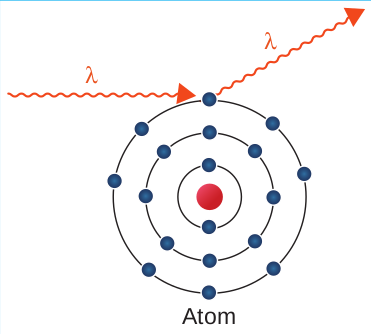
\includegraphics[width=0.7\linewidth]{images/rayleigh.png}
	\caption{Dispersión elástica\cite{khan2014the}}
	\label{fig:rayleigh}
\end{figure}
En este caso, el átomo se mueve solo lo suficiente para conservar el momento lineal. Por lo tanto, la contribución a la energía depositada por este proceso es despreciable. La contribución de este proceso al coeficiente másico de atenuación es despreciable a energías superiores a $10 keV$, que es mucho menor al rango de energía usado en radioterapia, por lo que no será tenido en cuenta.  \\

Por otro lado, el segundo tipo de dispersión es el denominado \textit{efecto Compton}. En este, un fotón incidente en un átomo interactúa de forma no elástica con un electrón, que se asume libre y estacionario, impartiendo cierta energía en él. Para que este proceso suceda, la energía de ligadura del electrón al átomo debe ser mucho menor a la energía del fotón incidente. Este proceso se ve ilustrado en la figura \ref{fig:compton}.\\
\begin{figure}[H]
	\centering
	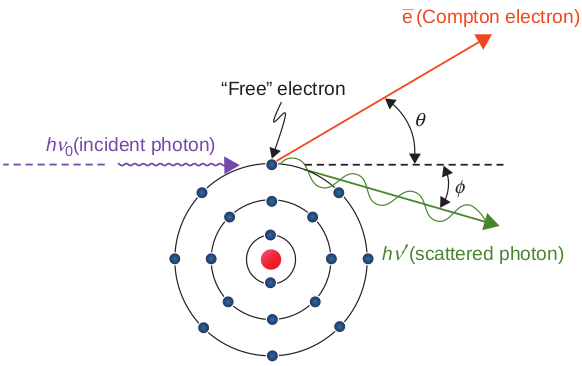
\includegraphics[width=0.7\linewidth]{images/compton.png}
	\caption{Dispersión no elástica- Efecto Compton \cite{khan2014the}}
	\label{fig:compton}
\end{figure}
En este proceso, el electrón es desligado del átomo y obtiene cierto momento en dirección $\theta$ con respecto a la dirección del fotón incidente. De la misma manera, el fotón es dispersado un ángulo $\phi$. \\

Este mecanismo puede ser estudiado desde la cinemática de la colisión de dos partículas relativistas. A partir de la conservación de energía y momento, es posible deducir las condiciones 
\begin{equation}
E=h \nu_{0} \frac{\alpha(1-\cos \phi)}{1+\alpha(1-\cos \phi)},
\end{equation}
\begin{equation}
h \nu^{\prime}=h \nu_{0}=\frac{1}{1+\alpha(1-\cos \phi)},
\end{equation}
\begin{equation}
\cot \theta=(1+\alpha) \tan \phi / 2,
\end{equation}
donde $h\nu_0$ es la energía del fotón incidente, $h\nu'$ es la energía del fotón dispersado, $E$ es la energía del electrón liberado y $\alpha=h\nu_0/m_0c^2$ con $m_0$ la masa en reposo del electrón. \\

Ahora, la probabilidad de que suceda un evento de este tipo puede calcularse mediante la sección eficaz del proceso. Esta viene dada por la fórmula de \textit{Klein-Nishina}, que expresa que la sección eficaz diferencial para este proceso es
\begin{equation}
\label{eqn:KleinNishina}
\frac{d_{e} \sigma}{d \Omega_{p}}=\frac{r_{0}^{2}}{2}\left(\frac{h \nu^{\prime}}{h \nu}\right)^{2}\left(\frac{h \nu}{h \nu^{\prime}}+\frac{h \nu^{\prime}}{h \nu}-\sin ^{2} \phi\right),
\end{equation}
donde $r_0=e^2/m_0c^2$ es el radio clásico del electrón.\\

La sección eficaz total por electrón bajo el modelo de Klein-Nishina se puede obtener integrando la ecuación \eqref{eqn:KleinNishina} sobre los posibles ángulos de dispersión del fotón, así
\begin{equation}
\begin{split}
_{e}\sigma&=2 \pi \int_{\phi=0}^{\pi} \frac{d_{e} \sigma}{d \Omega_{\phi}} \sin \phi d \phi\\
&=2 \pi r_{0}^{2}\left\{\frac{1+\alpha}{\alpha^{2}}\left[\frac{2(1+\alpha)}{1+2 \alpha}-\frac{\ln (1+2 \alpha)}{\alpha}\right]+\frac{\ln (1+2 \alpha)}{2 \alpha}-\frac{1+3 \alpha}{(1+2 \alpha)^{2}}\right\}.
\end{split}
\end{equation}
\\

Esta sección eficaz total por electrón es independiente del número atómico($Z$) del material con el que la radiación está interactuando,
\begin{equation}
	_{e}\sigma\propto Z^0,
\end{equation}
dado que no se está considerando que el electrón esté ligado al núcleo. De esta manera, la sección eficaz total por átomo con número atómico $Z$, viene dada por 
\begin{equation}
	_{a}\sigma=Z\cdot _{e}\sigma,
\end{equation}
y en consecuencia, el coeficiente de atenuación másico asociado al efecto Compton viene dado por 
\begin{equation}
	\frac{\sigma_c}{\rho}=\frac{N_{A}Z}{A}  _{e}\sigma,
\end{equation} 
donde $N_A$ es el número de Avogadro, $A$ es el peso molecular de los átomos del material y $\rho$ su densidad.\\

\textbf{Efecto Fotoeléctrico}\\

El efecto fotoeléctrico es el fenómeno en el cual un fotón incidente de radiación es absorbido por un átomo, y en consecuencia un electrón es liberado de este. En este proceso, toda la energía del fotón incidente $h\nu$ es transferida al electrón, que al final del proceso habrá adquirido una energía cinética de $T=h\nu-E_b$, donde $E_b$ es la energía de enlace del electrón al átomo. En este fenómeno es necesaria la presencia del núcleo atómico para lograr una conservación de momentos en el proceso. \\

Además del electrón liberado de la ligadura con el átomo, otros efectos secundarios pueden surgir a partir de esta interacción. Cuando el electrón es expulsado del átomo, esté deja un espacio libre que puede ocupar un electrón de una capa superior, y en este proceso de transición se producen rayos X característicos. También, esta energía liberada por la transición atómica puede ser absorbida por otro electrón en un nivel energético superior, lo que provoca que éste también sea liberado, en cuyo caso se denomina un \textit{electrón Auger}. Este proceso se ilustra en la figura \ref{fig:fotoelectrico}\\
\begin{figure}[H]
	\centering
	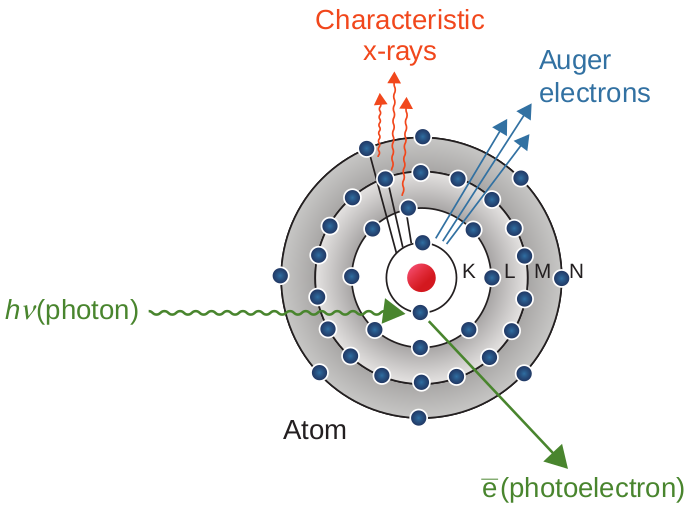
\includegraphics[width=0.7\linewidth]{images/fotoelectrico.png}
	\caption{Efecto fotoeléctrico \cite{khan2014the}}
	\label{fig:fotoelectrico}
\end{figure}

La probabilidad de que la interacción de efecto fotoeléctrico ocurra depende del numero atómico del material y de la energía del fotón incidente. Es posible describir aproximadamente su efecto sobre el coeficiente de atenuación mediante la sección eficaz por interacción
\begin{equation}
	\frac{\tau}{\rho}\propto \frac{Z^n}{E^m},
\end{equation} 
donde $Z$ es el número atómico del material, $E$ es la energía del fotón incidente, y $n$ y $m$ son números dependientes de la energía. Particularmente, $n\approx 4$ a $0.1 MeV$ aumentando gradualmente a $n\approx4.6$ a $3 MeV$ y $m\approx3$ a $0.1 MeV$ decreciendo a $m\approx1$ a $5 MeV$.\\

\textbf{Producción de pares}\\

Finalmente, si la energía de los fotones es superior a $1.02 MeV$ se puede producir interacción por producción de pares. En este proceso el fotón incidente interactúa con el campo electromagnético producido por el núcleo, produciéndose un par electrón-positrón, como se ilustra en la figura \ref{fig:Pares}. Para que este proceso suceda es necesario que el electrón tenga como mínimo la energía en reposo de dos electrones, que es de $0.511 MeV$. En este caso tenemos como ecuación de conservación de energía
\begin{equation}
	E=2m_0c^2+T^{+}+T^{-},
\end{equation}
donde $T^{+}$ es la energía del positrón y $T^{-}$ es la energía del electrón.\\

\begin{figure}[H]
	\centering
	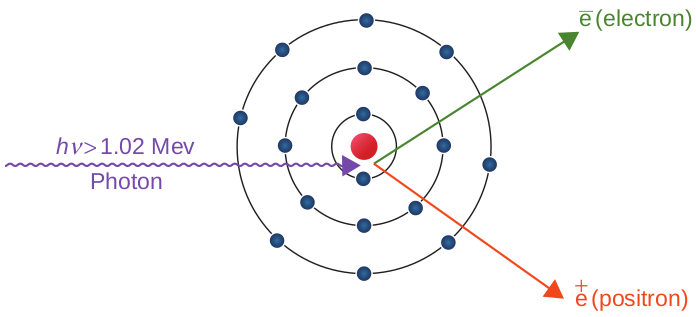
\includegraphics[width=0.7\linewidth]{images/produccionPares.png}
	\caption{Producción de pares \cite{khan2014the}}
	\label{fig:Pares}
\end{figure}

La probabilidad de que este suceso ocurra puede cuantificarse mediante la sección eficaz diferencial de Bethe y Heitler, que predice 
\begin{equation}
	d_{p}\kappa=\frac{\sigma_0 Z^2 P}{h\nu -2m_0c^2}dT^{+}, 
\end{equation}
denotando por $\sigma_0=r_{0}^2/137$ y $P$ una función de $E$ y $Z$, con lo cual la sección eficaz por átomo se calcula como
\begin{equation}
	_{p}\kappa=\sigma_0Z^2\overline{P},
\end{equation}
donde $\overline{P}$ es el promedio de la función $P$ sobre el intervalo de energía estudiado.\\

De esta manera, este proceso contribuye en el coeficiente de atenuación másico como
\begin{equation}
	\frac{\kappa}{\rho}=_{p}\kappa\frac{N_A}{A}.
\end{equation}.

Juntando todas las contribuciones por los diferentes procesos de interacción se obtiene un coeficiente de atenuación másico total $\mu/\rho$
\begin{equation}
	\frac{\mu}{\rho}=\frac{\sigma_c}{\rho}+\frac{\tau}{\rho}+\frac{\kappa}{\rho},
\end{equation}
que describe la capacidad de atenuación de determinado material ante la radiación.

En la figura \ref{fig:importanciaRelativa} se muestra la importancia relativa de estos tres efectos dependiendo del número atómico efectivo del material y la energía del haz. Aquí las curvas muestran los puntos donde los efectos colindantes tienen la misma sección eficaz.

\begin{figure}[H]
	\centering
	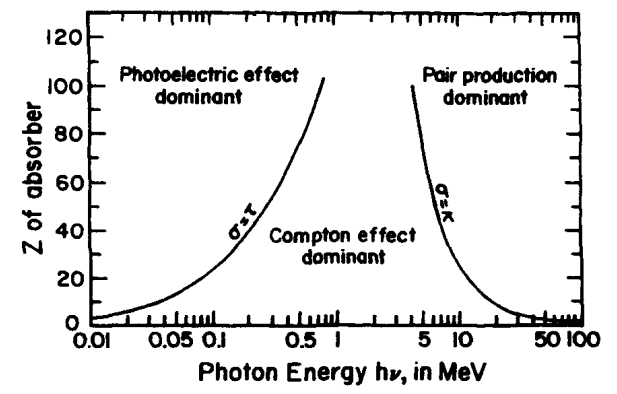
\includegraphics[width=0.7\linewidth]{images/importanciaRelativa.png}
	\caption{Importancia relativa de los tres principales tipos de interacción de fotones con la materia \cite{Attix1986}}
	\label{fig:importanciaRelativa}
\end{figure}

Así se evidencia que las interacciones más importantes de la radiación con agua en el régimen de energías de la radioterapia son las dispersiones Compton, seguidas de las contribuciones por producción de pares y finalmente, con un aporte bajo, las interacciones por efecto fotoeléctrico.  \\

\subsection{Interacción de partículas cargadas}

Las partículas cargadas, como los electrones o protones, interactúan con la materia de manera diferente a las partículas sin carga, como el fotón o neutrón. Una partícula sin carga podría pasar por la materia sin interactuar con ningún átomo y conservar toda su energía, o bien interactuar una o más veces, perdiendo su energía en el proceso. Por el contrario, una partícula cargada, al estar completamente rodeada de su campo columbiano, interactúa con cada átomo cercano a su trayectoria. Cada interacción individual transfiere una pequeña energía cinética de la partícula cargada, por lo que se puede considerar que ésta pierde energía de forma continua, en lo que es denominado la \textit{aproximación de frenado continuo}.\\

Para describir cuantitativamente el fenómeno de perdida energética continua por parte de una partícula cargada se usa la cantidad denominada \textit{poder de frenado}, $(dT/dx)_{T,Z}$, que se define como la energía promedio depositada por unidad de longitud por una partícula con energía cinética $T$ mientras se desplaza en un medio con número atómico $Z$. Si esta cantidad se divide por la densidad $\rho$ del material, se denomina el \textit{poder de frenado másico}.\\

Este poder de frenado puede separarse en dos componentes, 
\begin{equation}
	\frac{dT}{\rho dx}=\left(\frac{dT}{\rho dx}\right)_c+\left(\frac{dT}{\rho dx}\right)_r,
\end{equation}   
en donde el primer término representa perdidas de energía de la partícula por colisiones en interacciones directas de los campos de coulomb y el segundo representa perdida de energía por procesos radiativos, como el \textit{bremsstrahlung}.\\

El primer término puede ser aproximado mediante la fórmula de Bethe-Bloch, que para partículas pesadas como los protones expresa
\begin{equation}
	\left(\frac{d T}{\rho d x}\right)_{c}=2 k\left[\ln \left(\frac{2 m_{0} c^{2} \beta^{2}}{\left(1-\beta^{2}\right) I}\right)-\beta^{2} -\frac{C}{Z}\right],
\end{equation}
donde $\beta=v/c$ es el parámetro relativista de la velocidad, $I$ es el potencial de excitación medio del átomo, y $k,C$ son constantes. Y para partículas ligeras como electrones
\begin{equation}\left(\frac{d T}{\rho d x}\right)_{c}=k\left[\ln \left(\frac{\tau^{2}(\tau+2)}{2\left(I / m_{0} c^{2}\right)^{2}}\right)+F^{-}(\tau)-\delta-\frac{2 C}{Z}\right],\end{equation}
donde $\tau=T/m_0c^2$ y 
\begin{equation}F^{-}(\tau) \equiv 1-\beta^{2}+\frac{\tau^{2} / 8-(2 \tau+1) \ln 2}{(\tau+1)^{2}}.\end{equation}\\

Y finalmente, en el caso de partículas ligeras el término radiativo del poder de frenado puede ser aproximado por 
\begin{equation}\left(\frac{d T}{\rho d x}\right)_{r}=\sigma_{0} \frac{N_{A} Z^{2}}{A}\left(T+m_{0} c^{2}\right) \bar{B},\end{equation}
donde $\sigma_0=\frac{1}{137}(e^2/m_0c^2)^2$ y $\bar{B}$ es una función que varía lentamente con $Z$ y $T-$.

\section{Medidas de radiación ionizante}
Teniendo en cuenta que la radiación ionizante es particularmente peligrosa en tejidos biológicos cuando no se tiene suficiente control sobre ella, es necesario desarrollar un sistema de medida que permita describir cuantitativamente los efectos en la que un haz con cierta energía interactúa con la materia que atraviesa.\\

En primer lugar, es posible caracterizar un haz con su \textit{fluencia de partículas},denotada por $\Phi $, que se define como la cantidad diferencial dada por el cociente $dN$ por $da$, donde $dN$ es la cantidad esperada de partículas del haz que atraviesan una esfera imaginaria de sección transversal $da$.
\begin{equation}
\Phi=\frac{dN}{da}.
\end{equation}   
Con esta cantidad se puede definir la \textit{densidad de flujo}, denotada por $\phi$ como la fluencia de partículas $\Phi$ por unidad de tiempo
\begin{equation}
\phi=\frac{d\Phi}{dt}.
\end{equation}
Además, se define la \textit{fluencia de energía}, denotada por $\Psi$, como el valor esperado de energía de todas las partículas del haz que atraviesan una esfera imaginaria de sección transversal $da$.
\begin{equation}
\Psi=\frac{dE}{da},
\end{equation}
y con esta se define la densidad de flujo de energía, denotada como $\psi$, como la fluencia de energía por unidad de tiempo
\begin{equation}
\psi=\frac{d\Psi}{dt}.
\end{equation}
Por otro lado, es posible establecer unidades de medida para cuantificar la interacción de un haz con la materia. Las principales unidades de medida se presentan a continuación\\

\noindent
\textbf{Kerma($K$)}\\

Se define como la cantidad de energía cinética inicial de las partículas cargadas (electrones o positrones) que son liberadas por partículas sin carga (fotones) por unidad de masa
\begin{equation}
K=\frac{dE_{tr}}{dm},
\end{equation}
el kerma tiene unidades de $J/Kg$, denominada también Gray (Gy), ($1J/kg=1Gy$).
En el caso de un haz de fotones, es posible relacionar el kerma con la fluencia de energía mediante el \textit{coeficiente másico de transferencia de energía}, denotado por $(\mu_{tr}/\rho)_{E,Z}$, que es característico para cada material y la energía del haz, así
\begin{equation}
K=\Psi \left(\frac{\mu_{tr}}{\rho}\right)_{E,Z},
\end{equation} 
donde $\mu_{tr}$ es el \textit{coeficiente lineal de transferencia de energía}, con unidades $m^{-1}$ y $\rho$ es la densidad del material.\\

\noindent
\textbf{Dosis Absorbida($D$)}\\

Definimos la \textit{energía impartida}($\epsilon$) por radiación ionizante en un volumen finito $V$ que contiene una masa $m$ como
\begin{equation}
	\epsilon =R_{in}-R_{out}+\sum Q,
\end{equation}
donde $R_{in}$ es la energía de las partículas con carga y sin carga que entran en el volumen $V$, $R_{out}$ es la energía de estas mismas partículas que dejan el mismo volumen, y $\sum Q$ cuenta por la energía de las partículas en reposo en $V$.\\

De esta manera, la \textit{dosis absorbida}($D$) se define como el valor esperado de energía impartida en cierto material por unidad de masa
\begin{equation}
D=\frac{d\epsilon}{dm},
\end{equation}
la cual también tiene unidades de Gray(Gy).\\

\noindent
\textbf{Dosis equivalente($H$)}\\

La \textit{dosis equivalente}($H$) se usa para incluir en la mediada los efectos que tiene la radiación sobre cierto tipo específico de tejido, mediante la inclusión de un factor de calidad $Q$
\begin{equation}
H=Q\cdot D
\end{equation},
esta tiene unidades de Sievert(Sv), que tiene las mismas unidades dimensionales que el Gray.\\

\noindent
\textbf{Exposición($X$)}\\

La \textit{exposición}($X$) se define como el valor absoluto de la carga de un signo producida cuando todos los electrones liberados por fotones en procesos de ionización son detenidos completamente en aire por unidad de masa
\begin{equation}
X=\frac{dQ}{dm},
\end{equation}
y tiene unidades de $C/kg$.
\section{Principios de dosimetría}
\subsection{Equilibrio de partículas cargadas}
\subsection{Cámaras de ionización}
\subsection{Dosimetría con películas}
\section{Películas radiocrómicas}
Como fue mencionado anteriormente, la verificación de calidad de los tratamientos de radioterapia es de gran importancia para asegurar su efectividad. Es necesario comprobar que las distribuciones de dosis que se planean correspondan suficientemente con las distribuciones que recibe el paciente. Uno de los métodos más usados actualmente para realizar esta verificación sobre mapas de dosis en dos dimensiones es el uso de películas radiocrómicas.\\

Cuando las películas radiocrómicas son sometidas a radiación ionizante, estas sufren un cambio de color debido a un proceso químico de polimerización, adquiriendo una tonalidad diferente a la que tenían sin irradiar. El cambio de color que se produce es dependiente directamente de la dosis que se absorbe en cada punto. \\

Es posible medir este cambio de tonalidad de color de diferentes maneras, por ejemplo, midiendo con un escáner la intensidad de la luz que puede atravesarla. Con esta información de cambio de tonalidad y conociendo las dosis a las que fue sometida la película, es posible establecer una correlación que permita determinar la dosis absorbida en agua en otras circunstancias midiendo únicamente el cambio de coloración. \\

Uno de los primeros procesos radiocrómicos observados fue en 1826, cuando Joseph Niepce logró capturar la imagen de una ventana luego de dejar un papel cubierto con una solución fotosensible por un periodo de 8 horas, que dejó impregnada una imagen por medio de una polimerización de carbonos insaturados producidas por la absorción de energía del haz de luz.\\

El uso y desarrollo de estas sustancias fotosensibles fue evolucionando gradualmente. Por ejemplo, en 1965 McLauglin et al \cite{McLaughlin1965} reportaron el desarrollo de una solución de derivados de trifenilmetano que producía tintes por un proceso de radiosíntesis. Avances posteriores en materiales radiocrómicos estuvieron liderados por el NIST (National Institute of Standards and Technology), y en sus versiones más tempranas eran útiles en rangos de dosis entre $10^3$ y $10^6$ Gy, por lo que su espectro de aplicación se limitaba a procesos industriales\cite{Williams2011}.\\

La transición al uso de sustancias radiocrómicas en aplicaciones no industriales se dio con la aparición de las primeras películas GAFchromic producidas por ISP Technology en 1986. Estás nuevas películas tenían una composición nueva que permitia tener transformaciones cromáticas al exponerse a dosis de apenas 5 Gy\cite{Williams2011}.\\


Desde entonces, a partir de la variación en la composición de la sustancia radiocrómica y su empaquetado, se han han venido refinando los modelos de películas disponibles. En la actualidad existen diversos tipos de películas radiocrómicas que son útiles en dosimetría en varios rangos de dosis y para diferentes propósitos. Se usan comúnmente para dosimetría relativa, teniendo un patrón de dosimetría absoluta obtenido por otro método, como medidas con cámaras de ionización. En el cuadro \ref{tab:Modelos} se muestran diferentes modelos de películas y los rangos de dosis en los que se pueden usar.\\
\begin{table}[h!]
	\centering
	\begin{tabular}{|c|c|}
		
		\hline 
		Modelo & Rango de dosis \\ 
		\hline 
		HD-V2 & 10-100Gy \\ 
		\hline 
		MD-V3 & 1-100Gy \\ 
		\hline 
		EBT-XD & 0.04-40Gy \\ 
		\hline 
		EBT2 & 0.01-30Gy \\ 
		\hline 
		EBT3 & 0.01-30Gy \\ 
		\hline 
		XR-QA2 & 0.1-20 mGy \\ 
		\hline 
	\end{tabular} 
\caption{Modelos de películas radiocrómicas}
\label{tab:Modelos}
\end{table}

En general, los modelos difieren en la estructura y composición de la película, lo que permite mejores propiedades de sensibilidad a la radiación en cierto rango o estabilidad y uniformidad en el proceso de lectura. Por lo general, la películas consisten de una capa activa que contiene la sustancia radiocrómica y sus respectivos aditivos, encapsulada en capas de poliéster que las soportan y protegen del exterior. La estructura de diversos modelos se presenta en la figura \ref{fig:Estructuras}. Las placas más usadas en el contexto de verificación de radioterapia son las de la linea EBT.\\
\begin{figure}[H]
	\centering
	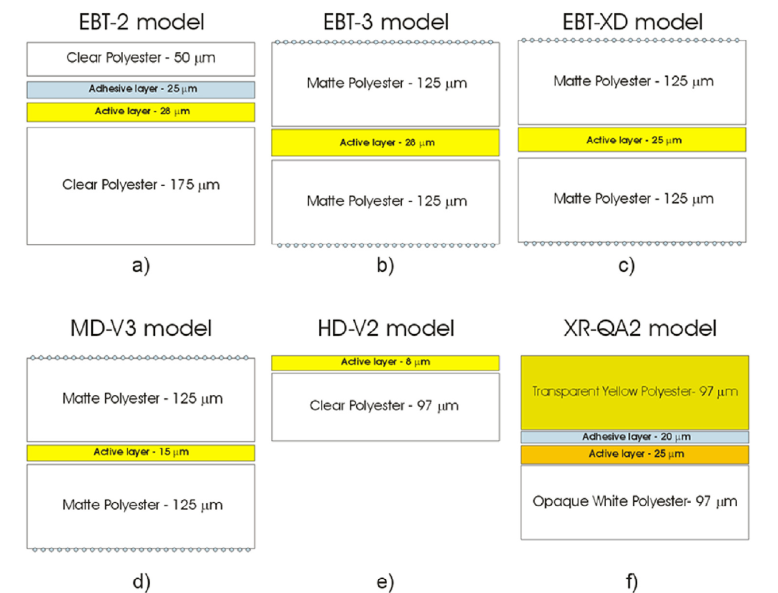
\includegraphics[width=\linewidth]{images/modelos.png}
	\caption{Estructuras de películas radiocrómicas de diferentes modelos. Tomada de \cite{Devic2016}}
	\label{fig:Estructuras}
\end{figure}

La capa activa está compuesta generalmente de cristales de poliacetilenos\cite{Williams2011}, particularmente de diacetelinos($C_4H_2$), que tras la exposición a la radiación o altas temperaturas sufren un proceso de polimerización que, junto con los aditivos, le proporciona un color diferente a la película. Específicamente, el componente activo de las películas EBT es la sal de litio del ácido pentacosa-10,12-diyonic, que sufre una 1,4-polimerización de estado solido de primer orden como se evidencia en la figura \ref{fig:reaccion}.\\  

\begin{figure}[H]
	\centering
	\subfloat[Monomeros de diacetileno\cite{Beni2017}]{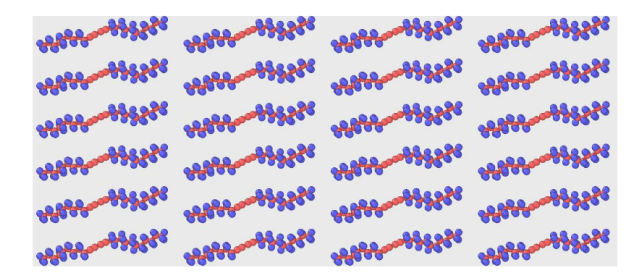
\includegraphics[width=0.5\textwidth]{images/diacetileno.png}\label{fig:diacetileno}}
	\hfill
	\subfloat[Reacción de polimerización\cite{Williams2011}]{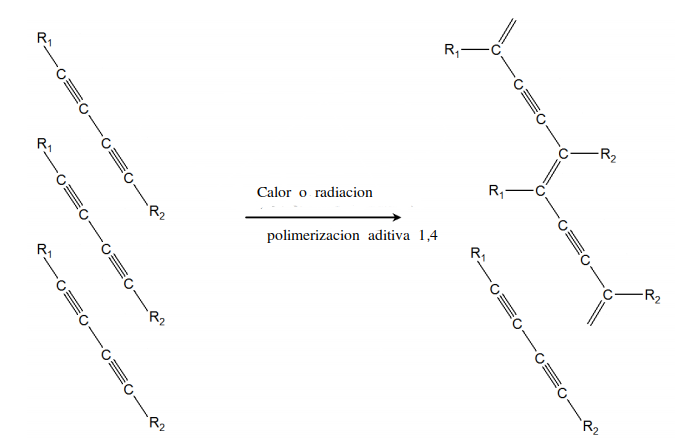
\includegraphics[width=0.5\textwidth]{images/reaccion.png}\label{fig:reaccion}}
	\caption{Polimerización de diacetilenos}
\end{figure}

El mayor cambio en coloración se produce casi instantáneamente después de la irradiación, sin embargo, la reacción puede tomar mucho más tiempo en completarse, estableciendo un tiempo de aproximadamente 24 horas para culminar este proceso \cite{Williams2011}. La velocidad de la reacción también depende de las condiciones de humedad\cite{LenMarroqun2018}, temperatura \cite{Rink2008} y exposición previa a las que está sometida la película\cite{NiroomandRad1998}. Por otro lado, estos cambios en la absorbancia de la película han sido mitigados en gran medida mediante aditivos en el componente activo, por lo que hoy en día con las modernas películas EBT3 las variaciones por estos factores resultan controlables siguiendo un protocolo sencillo de reproducibilidad. \\

También se han realizado estudios sobre la dependencia de la energía del haz en el proceso de coloración, encontrando que actualmente para las películas EBT3 la dependencia energética para energías mayores a 400 keV es mínima en un amplio rango de dosis absorbida\cite{Chemiski2010} . Además, para este tipo de placas se reporta un número atómico efectivo de $Z_{eff}=6.73$, que es muy cercano al número atómico efectivo del agua de $Z_{eff}=7.42$, por lo que la radiación interactúa de manera muy similar con ambos materiales. Lo anterior hace posible que las películas puedan ser usadas para medir dosis absorbida en agua sin factores de conversión adicionales.\\

Los cambios de absorbancia de una película cuando es sometida a la radiación pueden evidenciarse en una figura como la \ref{fig:AsorbanciaEBT3}, donde se muestra el espectro de absorción en el rango visible de una película EBT3 antes y después de ser irradiada con 5 Gy.\\
\begin{figure}[H]
	\centering
	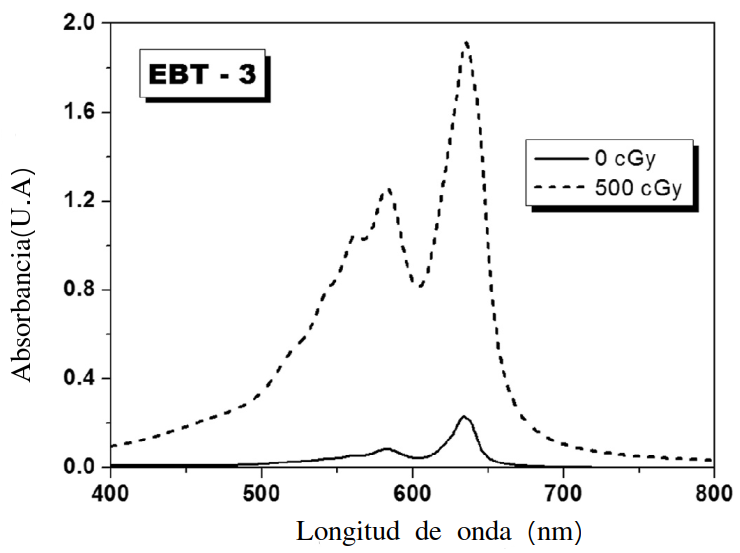
\includegraphics[width=0.7\linewidth]{images/absorbancia.png}
	\caption{Espectro de absorción de película EBT3. Tomada de \cite{Devic2016}}
	\label{fig:AsorbanciaEBT3}
\end{figure}

En esta se evidencia que la región del espectro donde se produce el mayor cambio de absorbancia es a rededor de 633 nm, en la región roja del espectro.\\

Para medir de manera práctica la absorbancia de una película irradiada existen diversos métodos. El más común es usar un escáner óptico, que proporciona una medida de la intensidad de la luz que la atraviesa. Un esquema de funcionamiento de un escáner común se muestra en la figura \ref{fig:escaner}.\\ 
\begin{figure}[H]
	\centering
	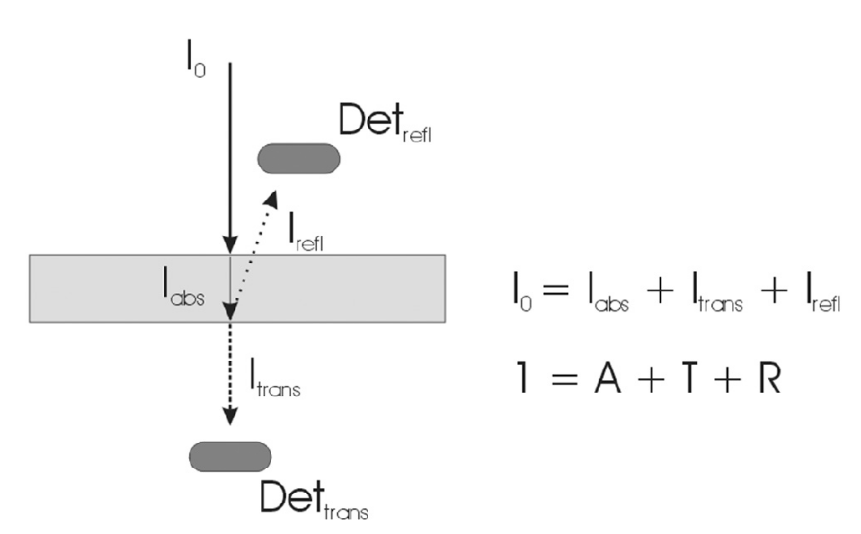
\includegraphics[width=0.7\linewidth]{images/escaner.png}
	\caption{Esquema de funcionamiento de escáner. Tomada de \cite{Devic2016}}
	\label{fig:escaner}
\end{figure}

El escáner proporciona una medida de cuánta luz deja pasar la película en cierto intervalo del espectro. Por ejemplo, en un escáner de transmitancia común  se proporciona información de cuánta intensidad transmitida $I_{tr}$ atravesó la película una intensidad inicial $I_0$. La forma más común en la que se almacena esta información en las aplicaciones consideradas es mediante una matriz RGB(red, green, blue) de 16 bits por canal. \\

Es decir, se almacena como 3 capas, cada una con información de una región del espectro analizado, el verde , el rojo o el azul, y cada pixel en cada capa adquiere un valor entre $0$ y $2^{16}-1$, que representa qué tanta intensidad de luz en el espectro fue medida en la posición del pixel. Concretamente, la información que proporciona la película resulta en tres matrices, una por cada color, que en cada entrada tiene un valor numérico que representa la cantidad de luz que se midió en la posición del pixel.\\

Con esta información es posible construir la \textit{transmitancia}$(T)$ en cada color de cada pixel, que se define como 
\begin{equation}
	T=\frac{I_{tr}}{I_0}=\frac{VP}{2^{16}-1},
\end{equation}
donde $VP$ es el valor del pixel medido por el escáner. Y con esta con esta se define la \textit{densidad óptica} $DO$ como 
\begin{equation}
	DO=-\log_{10}(T)=\log \frac{2^{16}-1}{VP}.
\end{equation}\\

Estos valores caracterizan los cambios de color de la película ante radiación medidos por un escáner, y serán útiles para establecer calibraciones que permitirán determinar planos de dosis.\\

En el proceso de escaneo existen varias variables que pueden modificar la transmitancia medida en cada pixel. Por ejemplo, se han reportado diferencias en las medidas de transmitancia dependiendo de la orientación de la película en el escáner\cite{mayers}. Este efecto es debido a que la luz del escáner es polarizada en una dirección y la película irradiada actúa como un polarizador que modifica la intensidad transmitida dependiendo de la orientación con respecto a la dirección de polarización.\\

Otra circunstancia que afecta la medida es la posición de la película en el escáner. Existe un efecto óptico en el sistema que provoca un aumento de la sensibilidad en el escáner cerca a los bordes laterales de este, que puede provocar una medida de más coloración, sobreestimando la dosis que recibió la película en esa región.\\

También se reportan cambios en la medida cuando la película se somete a cierto estrés mecánico\cite{Yu2006}, por ejemplo en el área de corte, dado que se altera la estructura y dimensiones de las capas que conforman la película. En tal caso, el efecto sobre la transmitancia medida es irregular, por lo que no se puede determinar precisamente cómo cambió la coloración cerca al corte.\\

Finalmente, también pueden existir defectos en la superficie de escaneo, como partículas de polvo o rayaduras, así como pixeles específicos del sensor del escáner que estén dañados. Todos estos factores influyen de alguna manera en la correlación final que se hace para obtener mapas de dosis. En caso de que su influencia sea importante, se deben aplicar ciertas correcciones en el procedimiento para obtener resultados adecuados.\\

Para obtener información de dosis a partir de la transmitancia medida en una película es necesario realizar un procedimiento de calibración. Este consiste en asociar las medidas de transmitancia en determinado canal de la película escaneada con las dosis que iniciaron el proceso de coloración que fueron medidas con otro mecanismo, por ejemplo, una cámara de ionización. La figura \ref{fig:EbtSin} muestra una película EBT2 sin irradiar y la figura \ref{fig:EbtCali} muestra la película irradiada con $11.1 ,  19.8, 22.9, 27.6, 37.1, 74.9, 102.4, 129.6, 151.9$ y $222.6 $ cGy.\\

\begin{figure}[H]
	\centering
	\subfloat[Película EBT2 sin irradiar]{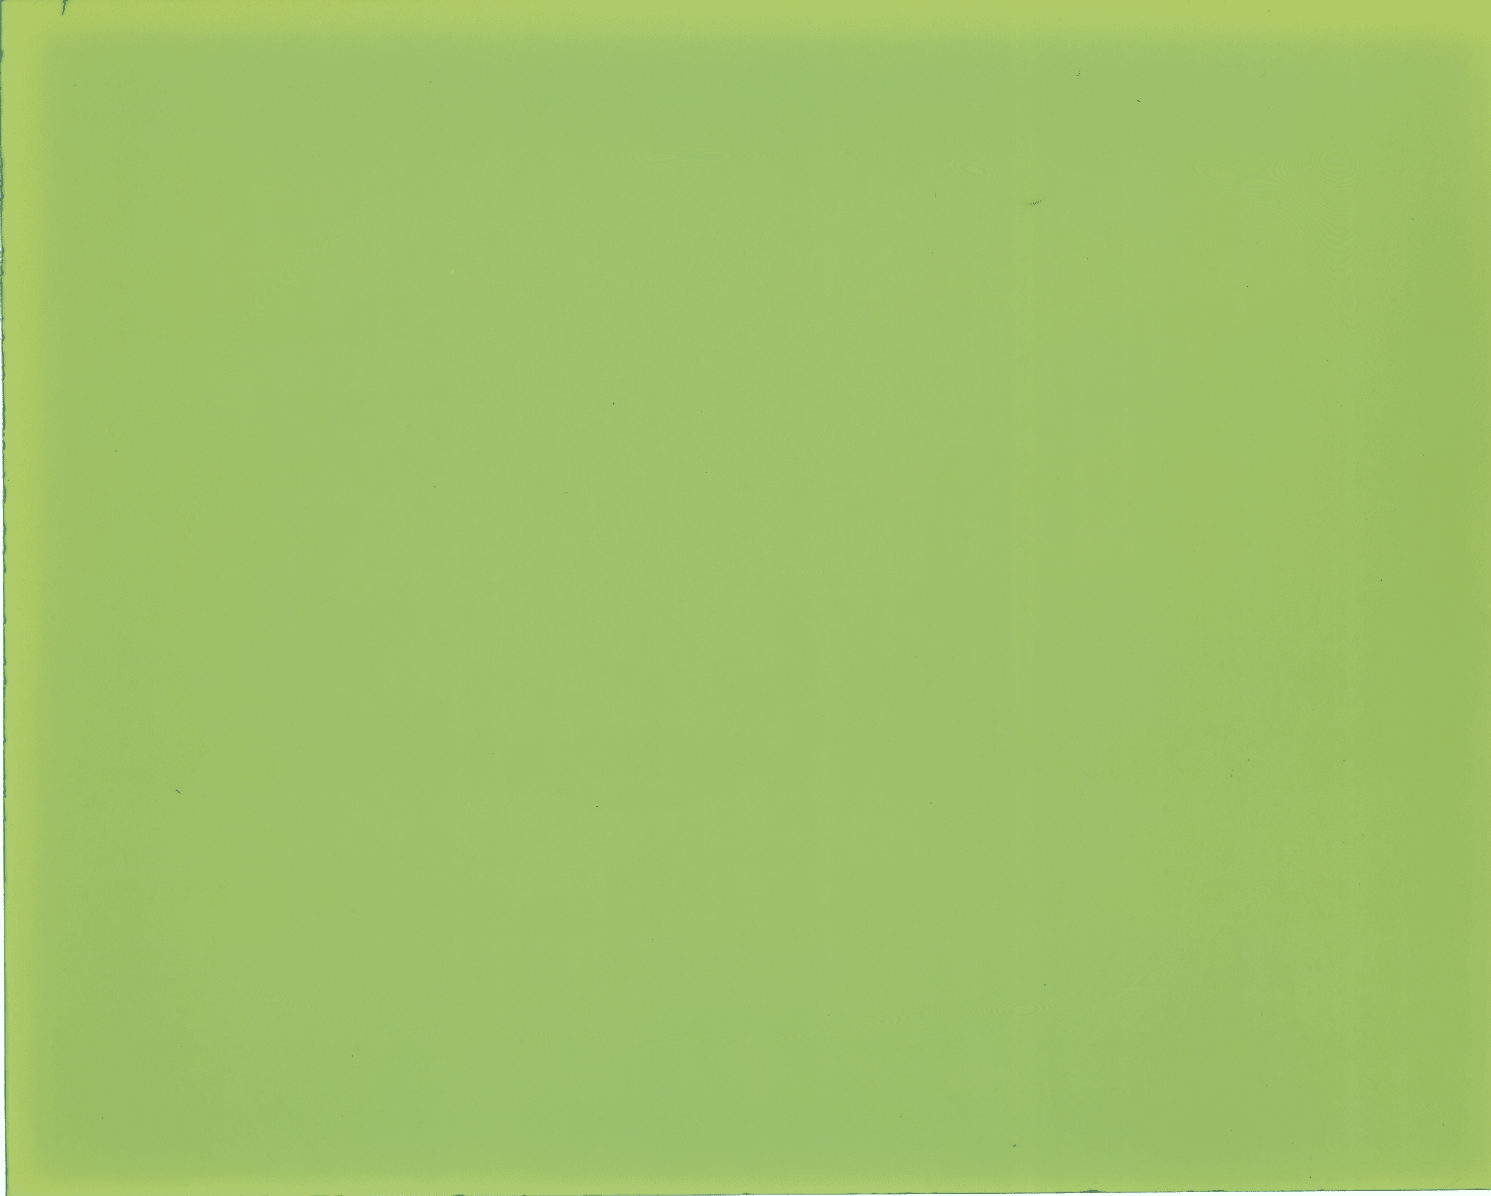
\includegraphics[width=0.5\textwidth]{images/fondoblancoLandscape-1.png}\label{fig:EbtSin}}
	\hfill
	\subfloat[Película EBT2 irradiada]{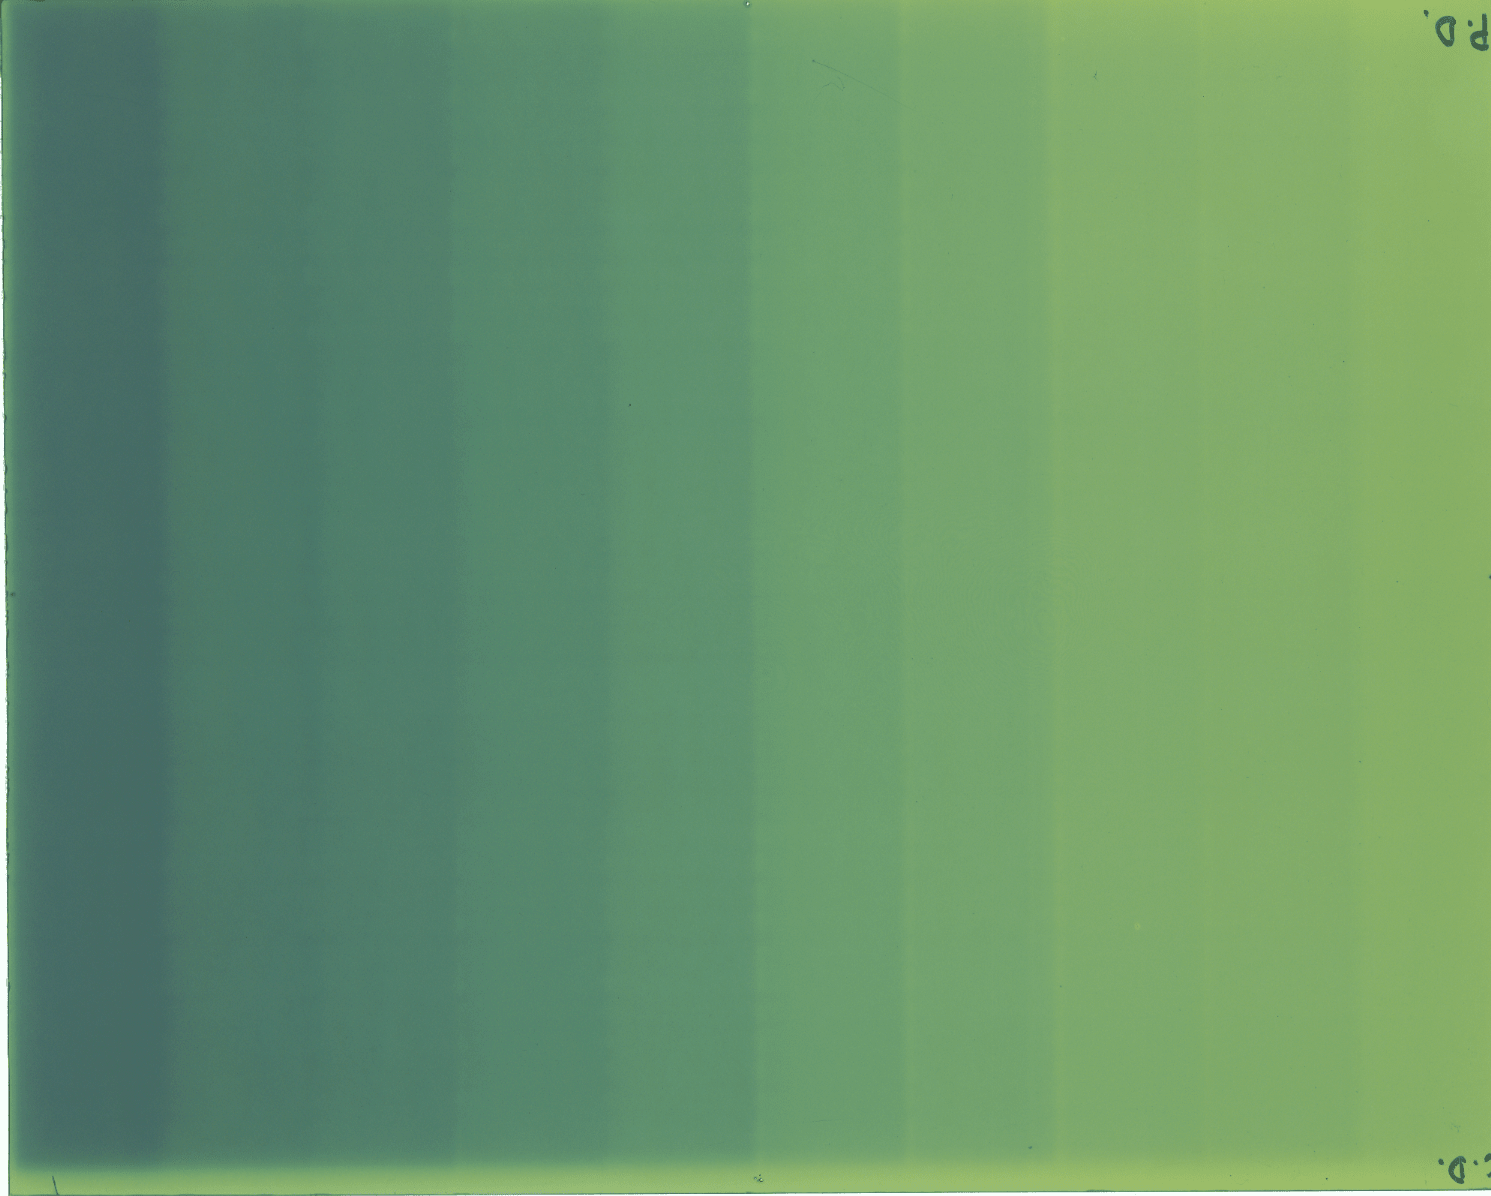
\includegraphics[width=0.5\textwidth]{images/calibracionSimpleLandscape.png}\label{fig:EbtCali}}
	\caption{Película EBT2 antes y después de irradiación}
\end{figure}

Promediando el valor de las transmitancias en cada canal de color en un región de interes(ROI) en cada una de las franjas, es posible obtener una función de respuesta de la película como la que se muestra en la figura \ref{fig:curvaRespuesta}. En esta imagen se evidencia que los canales de color en donde se presentan los mayores cambios son el rojo y el verde, por lo que son los más usados para obtener calibraciones.\\

\begin{figure}[H]
	\centering
	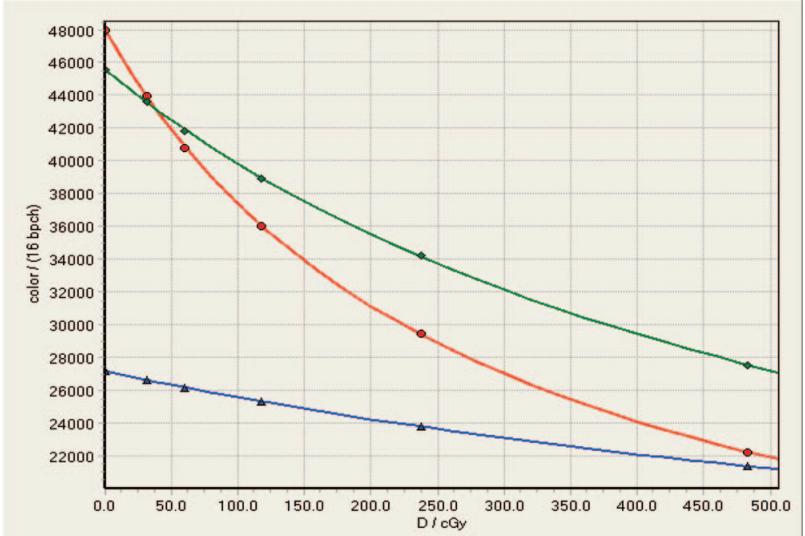
\includegraphics[width=0.5\linewidth]{images/respses.png}
	\caption{Curva de respuesta de película EBT2\cite{manualEBT2}}
	\label{fig:curvaRespuesta}
\end{figure}

Para determinar el cambio de coloración neto de la película se definen las cantidades de transmitancia neta ($netT$) en cada ROI como
\begin{equation}
	netT=T_{irr}-T_{bckg},
\end{equation}
donde $T_{irr}$ es el promedio de transmitancias en la ROI después de la irradiación y $T_{bckg}$ es el promedio de transmitancias en la ROI en la misma película antes de irradiar. Similarmente, se define la densidad óptica neta como 
\begin{equation}
	netOD=OD_{irr}-OD_{bckg},
\end{equation}
donde $OD_{irr}=-\log_{10}T_{irr}$ y $OD_{bckg}=-\log_{10}T_{bckg}$.\\

De esta manera, se construye una relación entre las transmitancias netas o las densidades ópticas netas con las dosis que produjeron la coloración y se ajusta una curva de calibración que permitirá interpolar valores para determinar mapas de dosis a partir de medir densidades ópticas. Un ejemplo de curva de respuesta y curva de calibración para un solo canal se muestra en la figura \ref{fig:Curvas}.

\begin{figure}[H]
	\centering
	\subfloat[Curva de respuesta\cite{Devic2016}]{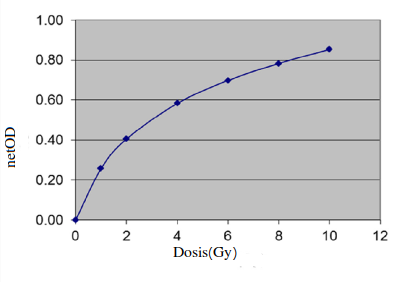
\includegraphics[width=0.5\textwidth]{images/curva1.png}\label{fig:resp}}
	\hfill
	\subfloat[Curva de calibración\cite{Devic2016}]{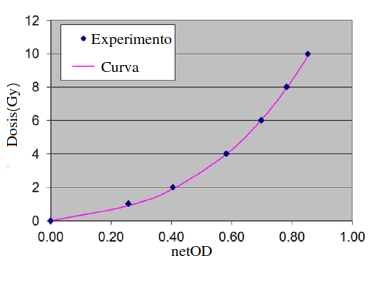
\includegraphics[width=0.5\textwidth]{images/curva2.png}\label{fig:caliv}}
	\caption{Curvas de calibración y respuesta}
	\label{fig:Curvas}
\end{figure}

En la literatura se han propuesto diversos tipo de curva de ajuste para modelar la relación de dependencia observada. Cada una es útil para cierto tipo de película y cierto rango de dosis, por lo que la elección de una en particular depende de la aplicación que se requiera. A continuación se muestran los tipos de funciones más usados\cite{Devic2016} \\

\begin{itemize}
\item\textbf{Función racional}\\
\begin{equation}
	D=\frac{A+B\cdot netT}{netT+D}
\end{equation}
\item\textbf{Función racional cuadrática}\\
\begin{equation}
D=\frac{A+B\cdot netT+C\cdot netT^2}{netT+D}
\end{equation}
\item\textbf{Función cuadrática}\\
\begin{equation}
D=A\cdot netOD^2+B\cdot netOD+C
\end{equation}
\item\textbf{Función cúbica}\\
\begin{equation}
D=A\cdot netOD^3+B\cdot netOD^2+C\cdot netOD +D 
\end{equation}

\item\textbf{Función inversa}\\
\begin{equation}
D=A+\frac{B}{netT-C}
\end{equation}

\item\textbf{Función exponencial}\\
\begin{equation}
D=A\cdot netOD+B\cdot netOD^n
\end{equation}
\end{itemize}

También se han propuesto diversas modificaciones y metodologías para aumentar la precisión de la dosis determinada por la calibración. Cada una de estas tiene en cuenta algún aspecto en particular que altere la medición y lo corrige de cierta manera. A continuación se presentan los principales métodos de corrección.\\


\textbf{Filtrado de las imágenes escaneadas\cite{Devic2005}\cite{Li2017}}\\

Para corregir inhomogeneidades de la película, así cómo irregularidades en la superficie del escáner y pixeles defectuosos se pueden implementar varias correcciones. La más sencilla de ellas es la aplicación de un filtro que elimine outliers de las imágenes, reemplazando su valor por un promedio de los pixeles más cercanos. También se puede escanear varias veces la misma imagen, para luego realizar un promedio ponderado entre ella, eliminando así ciertas irregularidades y reduciendo la incertidumbre teórica que se alcanza.\\

Por otro lado, es común usar un filtro adaptativo de Wiener para reducir el ruido de varias fuentes que puedan tener las imágenes. Este permite eliminar ruido interno producido en la imagen por escaner, como el ruido que se produce en los sensores CCD cuando se están midiendo transmitancias bajas.\\

\textbf{Corrección de efecto lateral} \\

En el caso de usar solo un canal de color para la calibración, en \cite{Crijns2013} se sugiere usar una modificación en la función usada para que tenga en cuenta el efecto de cambio de dosis cerca a los bordes laterales. En la figura \ref{fig:efectoLateral} se evidencia  un ejemplo de este efecto. Esta muestra el perfil de dosis obtenido de una película irradiada uniformemente con una dosis particular, sin embargo en los extremos de la película, los que están cercanos a la parte lateral de escáner, se evidencia una sobre-estimación en la dosis predicha. El efecto sobre la dosis calculada es mayor conforme la dosis aumenta.\\

\begin{figure}[H]
	\centering
	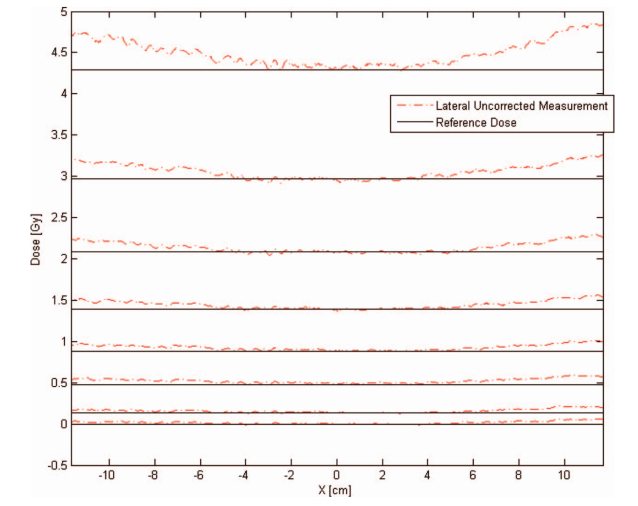
\includegraphics[width=0.9\linewidth]{images/efectoLateral.png}
	\caption{Ilustración del efecto de escaneo lateral para el canal rojo \cite{Crijns2013}}
	\label{fig:efectoLateral}
\end{figure}

Una manera de corregir este efecto es modificar la función de calibración modelando este comportamiento de sobre-estimación. Por ejemplo, si se usa una función racional como las mencionadas anteriormente, una posible modificación modelando el comportamiento del efecto mediante una función cuadrática que tenga como parámetro la variable de posición del escáner, quedando como nueva función
\begin{equation}
	T=T_{\infty}+\frac{T_0-T_{\infty}}{1+\frac{D}{\beta_{3}}}+\beta_{4}D+\beta_{5}X^2,
\end{equation}
donde $T_0, T_{\infty},\beta_{3},\beta_{4},\beta_{5}$ son ahora los nuevos parámetros de ajuste.\\


\textbf{Calibración multicanal}\\

Una manera ingeniosa de mejorar la precisión de las medidas, así como corregir cambios de color no debidos a la dosis absorbida, es usando la información de los tres canales de color como es propuesto en \cite{Micke2011} y expuesto más claramente en \cite{Li2017}. \\

Este método asume que la densidad óptica $(OD)$ en cualquier punto de la película es proporcional al grosor de la capa de material activo
\begin{equation}
	OD_{k}=u_{k}\cdot t \quad k=R,G,B
\end{equation} 
donde $u_k$ es el coeficiente de absorción de la capa activa en cada canal, que varía con la dosis absorbida, y $t$ es una medida adimensional asociada al espesor de la capa activa. Si $f_k$ es la curva de calibración que se está usando para modelar el comportamiento en cada canal, entonces 
\begin{equation}
\label{eqn:cass}
	D_k=f^{-1}(OD_k\cdot t).
\end{equation}

Como la dosis no puede depender del canal de color usado, es posible plantear un problema de optimización en el que variando $t$ se minimizen las diferencias de dosis obtenidas con cada canal, es decir resolver el problema
\begin{equation}
	\min_{t}\sum_{i,j=R,G,B}(D_i-D_j)^2.
\end{equation}

Usando la solución óptima a este problema $t_{opt}$, podemos usar \eqref{eqn:cass} para calcular la dosis en cada canal, y al final tomar el promedio de los resultados en los los tres canales.
\begin{equation}
	D=\frac{D_R+D_G+D_B}{3}
\end{equation}

\section{Análisis $\Gamma$}
Dada la complejidad que suponen ciertos tratamientos y la necesidad de asegurar que las dosis prescritas correspondan con gran precisión con las dosis entregadas en estos, se deben proponer formas cuantitativas para evaluar qué tanto corresponden entre sí dos mapas de dosis asociados a los planes. Esto se requiere, por ejemplo, cuando por diversas razones es necesario cambiar el algoritmo de cálculo de dosis que usa el sistema de planeación para calcular los planes. En tal caso, es necesario validar el reajuste con los planes previamente calculados, para asegurar que correspondan con las dosis prescritas.\cite{Winiecki2009}\cite{Li2011}\\

En este caso, se quiere validar que los planes calculados con el sistema de planeación correspondan con los que se ejecutan en tiempo real en la máquina. Esto dado que, en algunos casos, para planes complejos, las limitaciones de la máquina que no tiene en cuenta el sistema podrían generar distribuciones inciertas que afectan la efectividad del tratamiento.\\

En consecuencia, para propósitos de comparación de planes, se ha desarrollado una nueva cantidad denominada $\Gamma$. Si se desea comparar una distribución de dosis de referencia $D(\vec{r}_{c})$ con una distribución de dosis medida $D(\vec{r}_{m})$ entonces se define $\Gamma(\vec{r}_c,\vec{r}_m)$ para cada punto de referencia con respecto a cada punto de medida como 
\begin{equation}
\label{eqn:gamma}
\Gamma(\vec{r}_c,\vec{r}_m)=\sqrt{\frac{\abs{\vec{r}_c-\vec{r}_m}^2}{DTA^2}+\frac{\abs{D(\vec{r}_c)-D(\vec{r}_m)}^2}{DD^2\cdot D(\vec{r}_c)^2}},
\end{equation}
donde $\abs{\vec{r}_c-\vec{r}_m}$ es la distancia entre los puntos analizados en milímetros, ${\abs{D(\vec{r}_c)-D(\vec{r}_m)}}$ es la diferencia de dosis entre los puntos y $DTA$(Distance to Agreement) y $DD$(Dose diference) son parámetros para ajustar la calidad de la comparación. Teniendo estos valores, se define el valor de $\Gamma$ en cada punto de la distribución de referencia como el mínimo de estas cantidades evaluadas sobre los puntos en la distribución de mediada, es decir $\Gamma(\vec{r}_c)=\min_{m} \Gamma(\vec{r}_c,\vec{r}_m)$.\\

De esta manera, para $DTA$ y $DD$ fijos, se está buscando en la distribución medida el punto que está más cercano en una distancia de hasta $DTA$ y difiere en dosis hasta $DD$ con respecto a algún punto en la distribución de referencia. Parámetros usuales para realizar este análisis son $DTA=3 mm$ y $DD=3.3\%$, aunque para planes más complejos, con gradientes de dosis altos, se pueden usar parámetros menores, como $DTA=1 mm$ y $DD=1\%$.\\

Cada punto en la distribución de referencia pasa el test de comparación con la distribución medida si su $\Gamma(\vec{r}_c)<1$, lo que quiere decir que, bajo la definición de comparación de distribuciones, estas coinciden en un valor aceptable. Gráficamente, el significado de este test de ajuste entre distribuciones es representado en la figura \ref{fig:elipseGamma}, donde un punto en la distribución de referencia pasa el test si reside en la elipse  definida por la ecuación \eqref{eqn:gamma}.\\
\begin{figure}
	\centering
	\missingfigure[figwidth=\linewidth,figcolor=white]{Ellipse Gamma}
	\caption{Significado geométrico del test gamma }
	\label{fig:elipseGamma}
\end{figure}





